\chapter{AWG-9 RADAR}
\thumbtab{AWG-9}{2}
\minitoc
\cleardoublepage

\section{OVERVIEW}
% \subsection{MAIN MODES - OVERVIEW}
\begin{table}[h]
    \centering
    \caption{\textbf{Overview of AWG-9 Radar Modes}}
    \label{tab:awg9overview}
    \begin{tabular}{p{1.4cm} | p{1.2cm} | p{1.2cm} | p{1.2cm} | p{1cm} | p{1cm} | p{1.5cm}}
        \toprule
        & \multicolumn{2}{c |}{\blue{Pulse}} & \multicolumn{4}{c}{\blue{Pulse Doppler}} \\
        \midrule
        & \textbf{Pulse Search} & \textbf{P-STT} & \textbf{PD Search} & \textbf{RWS} & \textbf{TWS} & \textbf{PD-STT} \\
        \midrule
        \textbf{Range (approx.)} & 60 nm & 50 nm & 110 nm & 90 nm & 90 nm & 90 nm \\
        \midrule
        \textbf{AIM-7} & BRSIT & CW & \multicolumn{2}{c |}{BRSIT} & - & PD \\
        \midrule
        \textbf{AIM-54} & BRSIT & ACT & \multicolumn{2}{c |}{BRSIT} & Multi TGT & PD/ACT \\
        \bottomrule
    \end{tabular}
\end{table}

\subsection{MAIN MODES}
\begin{tableitemize}
    \blueitem{Pulse}{
    \begin{subitemize}
        \item \textbf{Basic Pulse w/o doppler filtering}
        \begin{itemize}
            \item Cannot be notched
            \item Ground Clutter
            \item Rudimentary Ground mapping
        \end{itemize}
        \item \textbf{Pulse Sub-Modes}
        \begin{itemize}
            \item \textbf{Pulse Search}
            \item \textbf{Pulse-STT}
        \end{itemize}
    \end{subitemize}}
    \blueitem{Pulse Doppler}{
    \begin{subitemize}
        \item \textbf{Doppler filter --> no ground returns}
        \begin{itemize}
            \item Susceptible to notching
            \item No ground clutter
            \item Greater range
            \item Advanced sub modes
            \item AIM-54 Guidance
        \end{itemize}
        \item \textbf{Pulse Doppler Sub-Modes}
        \begin{itemize}
            \item \textbf{PD Search}
            \item \textbf{RWS}
            \item \textbf{TWS}
            \item \textbf{PD-STT}
        \end{itemize}
    \end{subitemize}}
\end{tableitemize}

\clearpage

\section{PULSE MODES}

\subsection{PULSE SEARCH}
\begin{figure}[htbp]
    \centering
    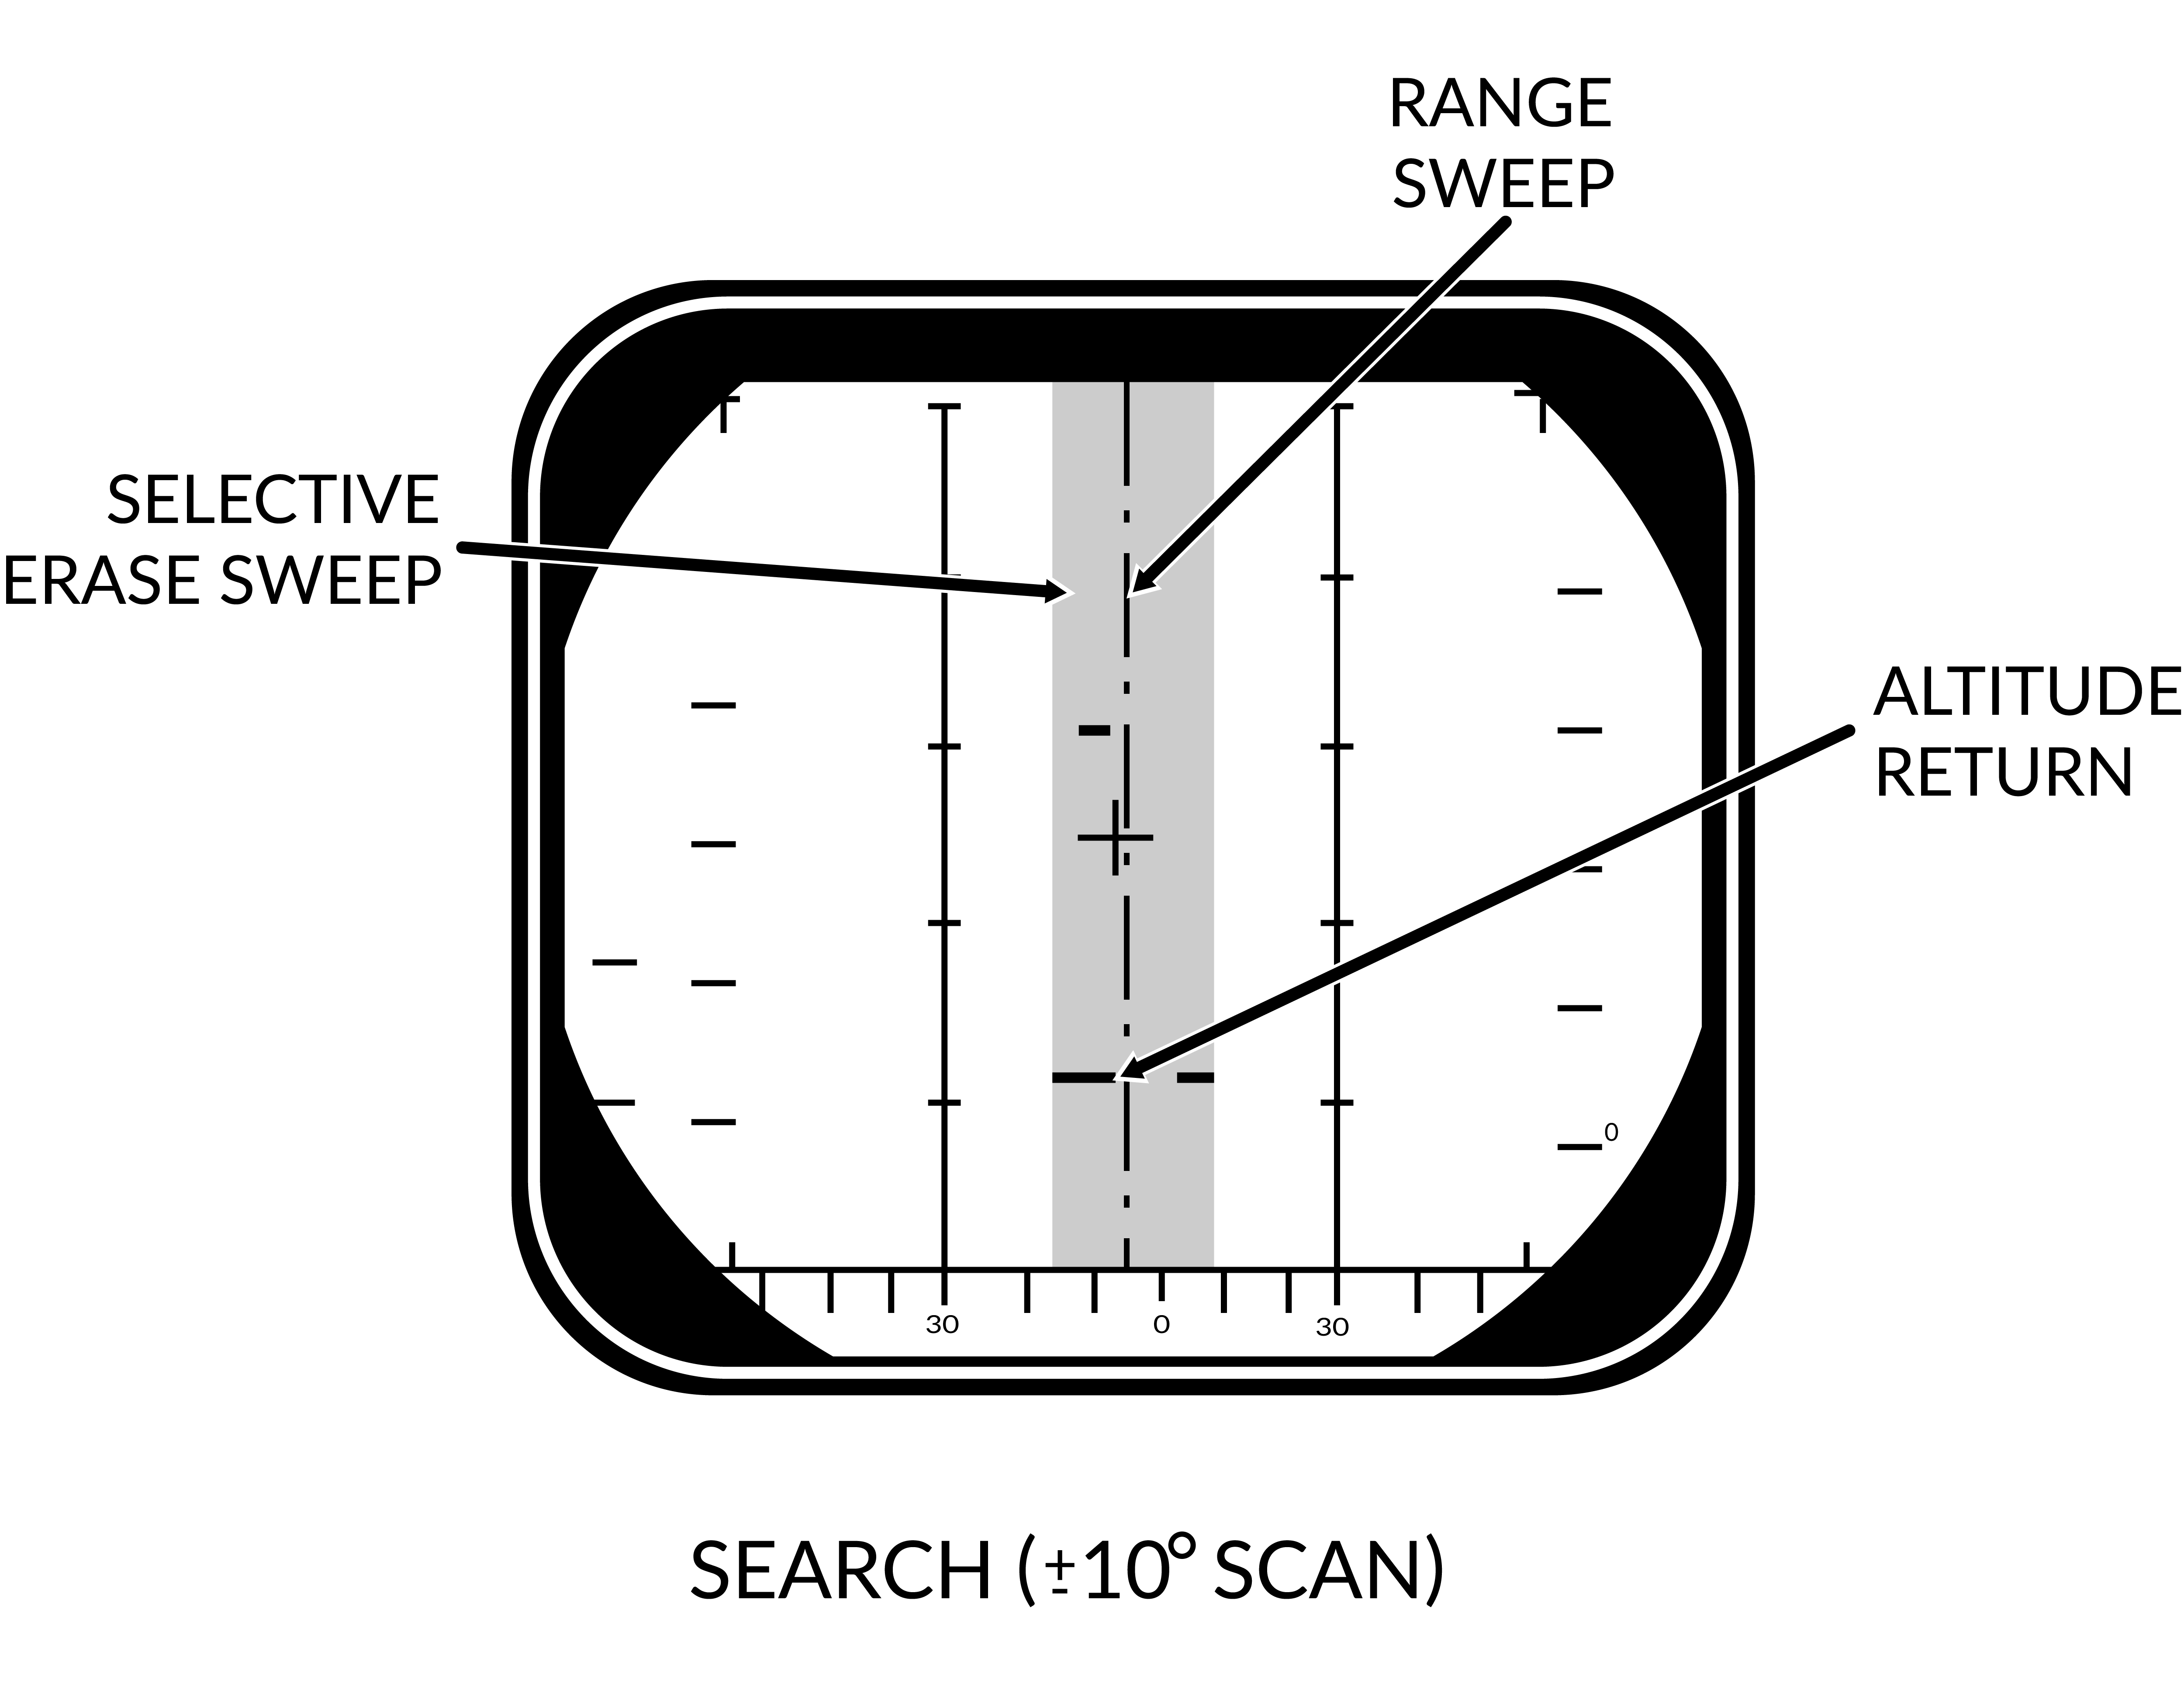
\includegraphics[width=0.8\linewidth]{PSEARCH.png}
    \caption{\textbf{DDD Format in Pulse Search Mode}}
    \label{fig:psearch}
\end{figure}
\begin{tableitemize}
    \blueitem{Pulse Search}{\textbf{Basic Mode} - AWG-9 does not use pulse doppler filtering

    \begin{subitemize}
        \item \textbf{Advantages}
        \begin{itemize}
            \item All aspect target detection
            \item Cannot be notched
            \item Rudimentary ground mapping
        \end{itemize}
        \item \textbf{Disadvantages}
        \begin{itemize}
            \item No ground return filtering 
            \item Lower range
        \end{itemize}
    \end{subitemize}}
    \blueitem{DDD}{
    \begin{subitemize}
        \item \textbf{Range/Azimuth}
        \item Visualization of radar and erase sweeps
    \end{subitemize}}
    \blueitem{TID}{
    \begin{subitemize}
        \item \textbf{No Information from Pulse}
        \item \textbf{Cannot guide AIM-54}
    \end{subitemize}}
\end{tableitemize}


\clearpage

\subsection{PSTT}
\begin{figure}[htbp]
    \centering
    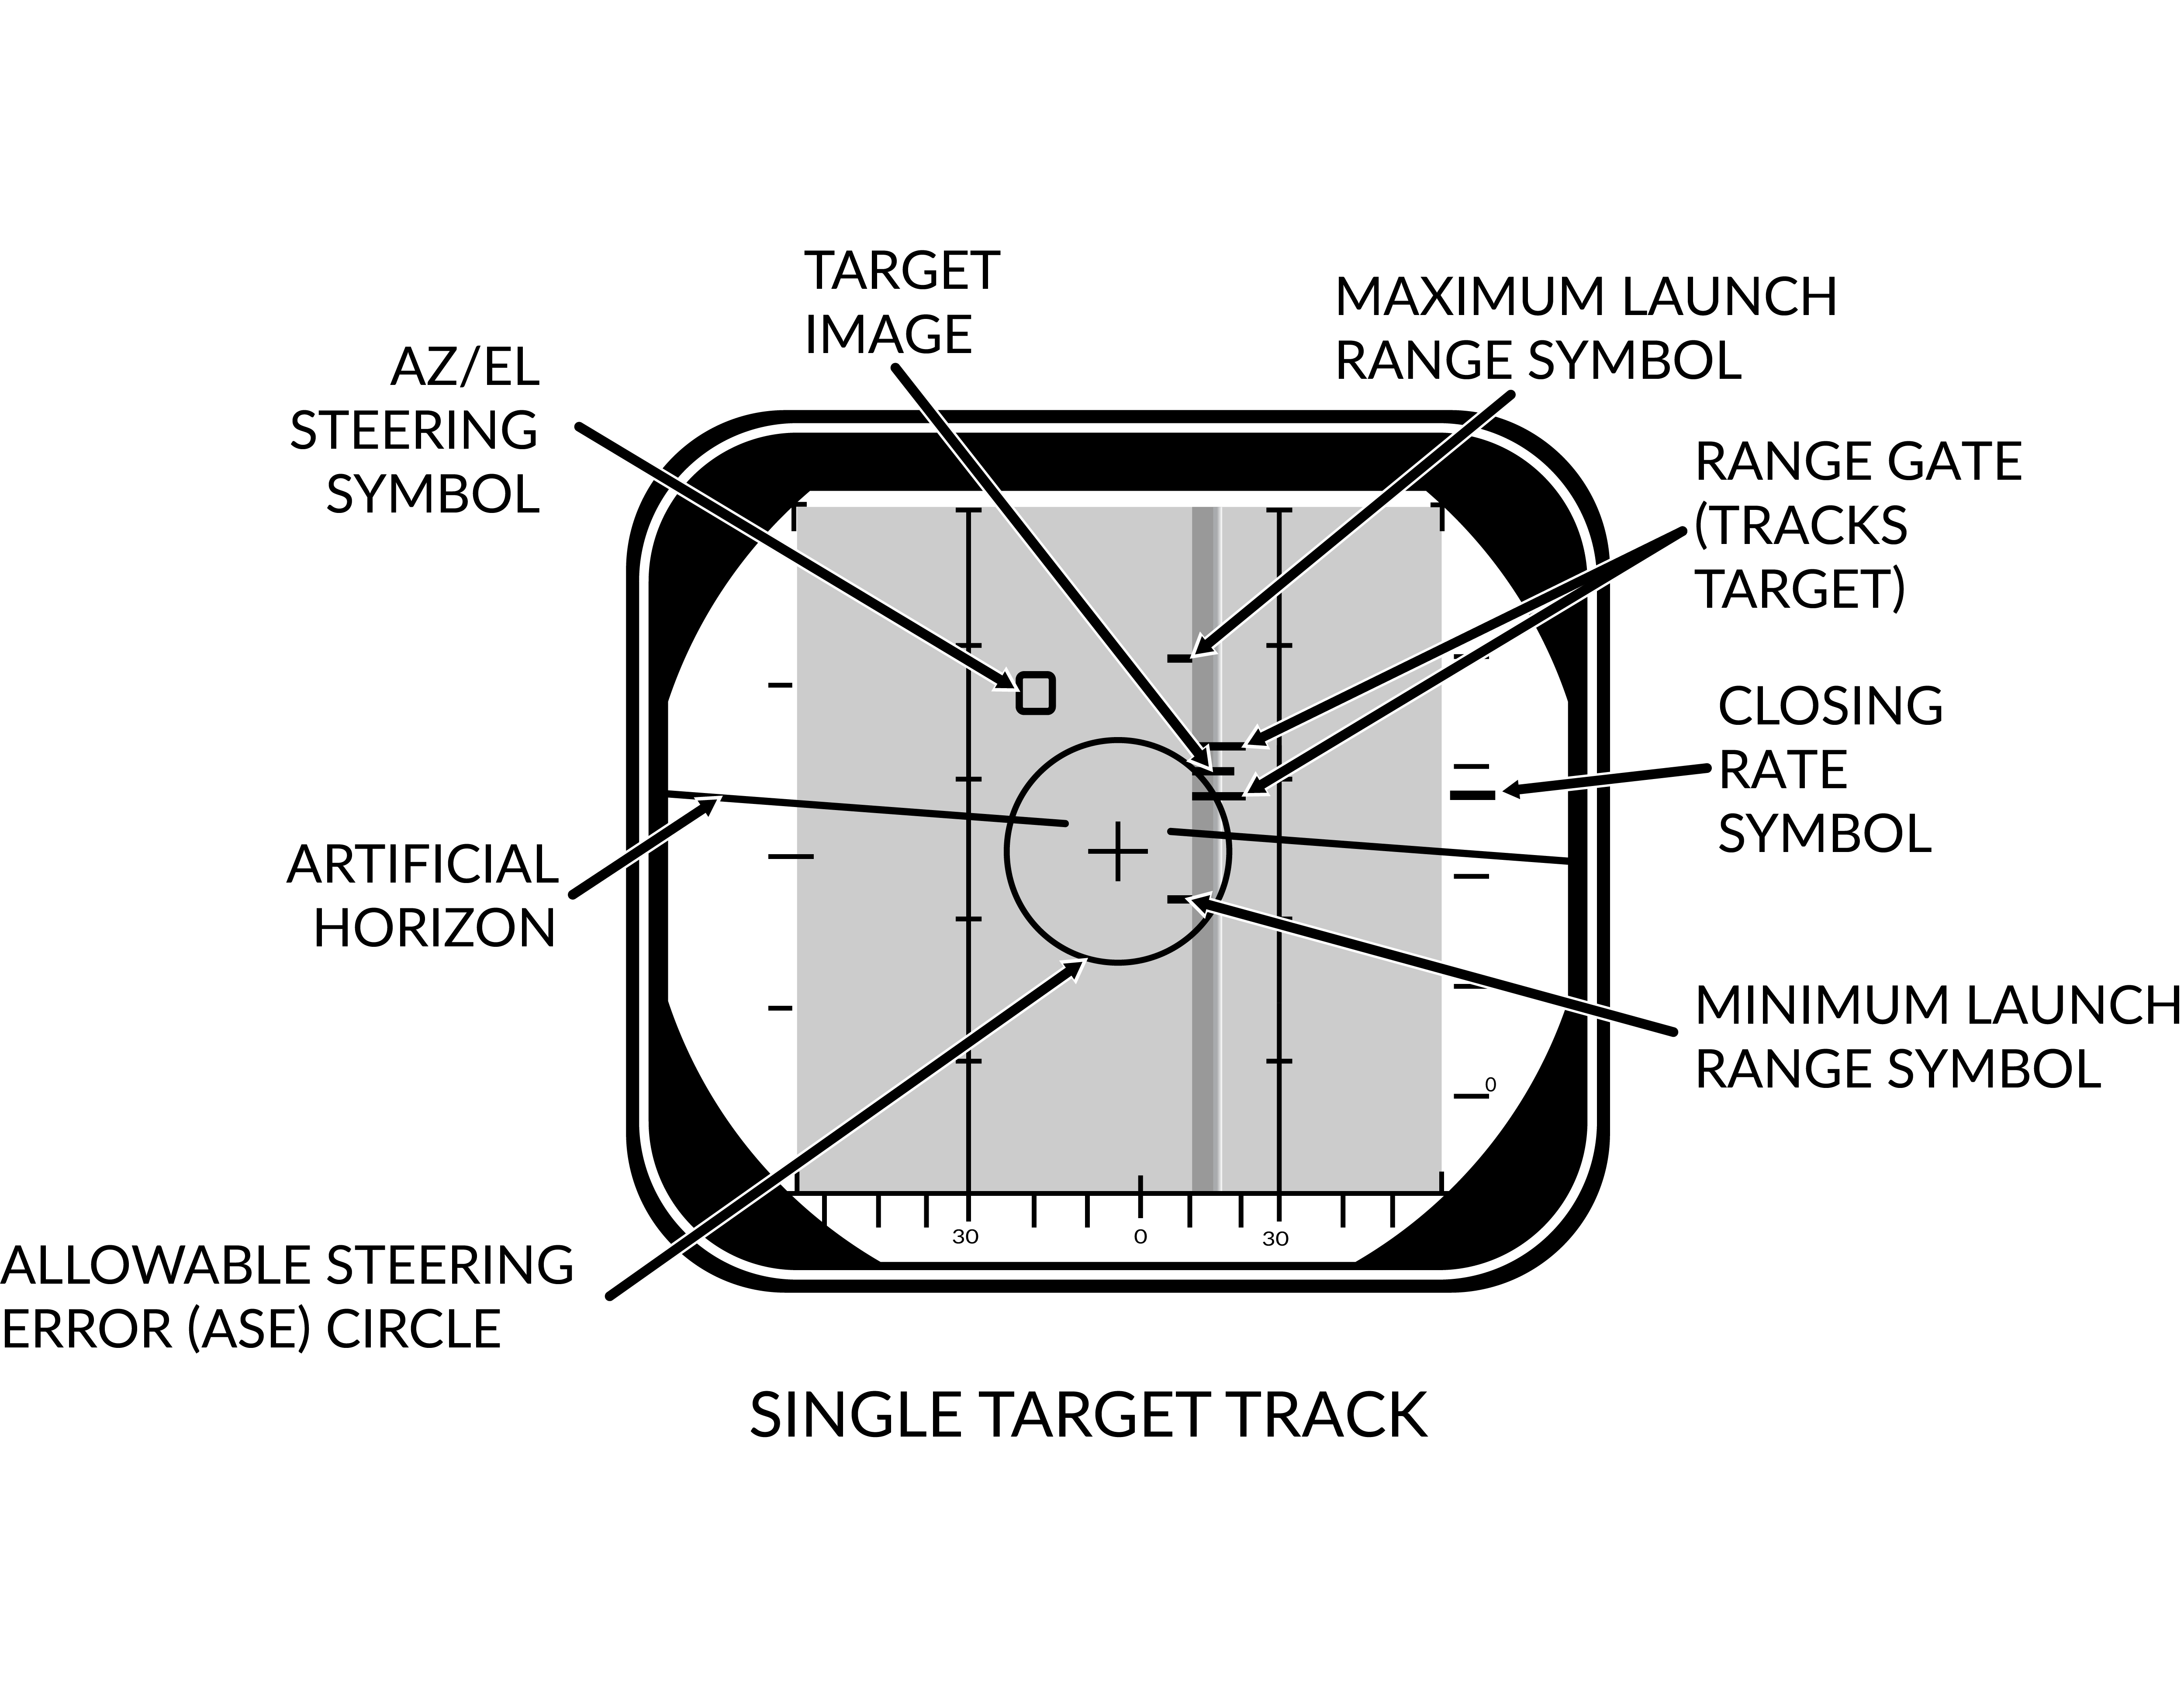
\includegraphics[width=0.90\linewidth]{PSTT.png}
    \caption{\textbf{DDD Format in PSTT Mode}}
    \label{fig:pstt}
\end{figure}
\begin{tableitemize}
    \blueitem{Pulse STT}{Lock Target w/o doppler filtering 
    \begin{subitemize}
        \item \textbf{Advantages} -- Cannot be notched
        \item \textbf{Disadvantages} -- Susceptible to ground clutter
    \end{subitemize}}
    \blueitem{DDD}{
    \begin{subitemize}
        \item \textbf{Track Indications}
        \begin{itemize}
            \item ANT TRK \& RDROT lights
            \item Tracking gates
            \item Closure rate
            \item Attack Symbology
        \end{itemize}
    \end{subitemize}}
\end{tableitemize}

\notebox{
    \begin{itemize}
        \item \textbf{PSTT Lock Affects Missile Logic}
        \begin{itemize}
            \item AIM-54 launched in \textbf{Active Launch Mode}
            \item AIM-7 launched in \textbf{CW Mode}
        \end{itemize}
    \end{itemize}
}

\clearpage

\subsection{PSTT ACQUISITION}
\begin{tableitemize}
    \blueitem{Pulse To PSTT}{
    \begin{subitemize}
        \item \textbf{Conditions}
        \begin{itemize}
            \item Pulse Search Mode selected
            \item RDR HCU Mode selected
        \end{itemize}
        \item \textbf{Lock Target}
        \begin{enumerate}
            \item Hold HCU Half-action
            \item Slew acquisition gates over desired Target on DDD
            \item HCU Full-Action to lock
        \end{enumerate}
        \item \textbf{Unlock Target}
        \begin{enumerate}[resume]
            \item HCU Half-action
        \end{enumerate}
    \end{subitemize}}
    \blueitem{TWS to PSTT}{
    \begin{subitemize}
        \item \textbf{Conditions}
        \begin{itemize}
            \item TWS Mode selected
            \item RDR HCU Mode selected
        \end{itemize}
        \item \textbf{Lock Target}
        \begin{enumerate}
            \item Hook Target on TID
            \item Press PSTT button on DDD Panel
        \end{enumerate}
        \item \textbf{Unlock Target}
        \begin{enumerate}[resume]
            \item HCU Half-action
        \end{enumerate}
    \end{subitemize}}
    \blueitem{ACM to PSTT}{
    \begin{subitemize}
        \item \textbf{Lock Target}
        \begin{enumerate}
            \item Select desired ACM Mode (Pilot or RIO)
            \item Place target in search volume through maneuvering
        \end{enumerate}
        \item \textbf{Unlock Target}
        \begin{enumerate}[resume]
            \item HCU Half-action
        \end{enumerate}
    \end{subitemize}}
    \blueitem{PDSTT to PSTT}{
    \begin{subitemize}
        \item \textbf{Conditions}
        \begin{itemize}
            \item Target PDSTT Locked
        \end{itemize}
        \item \textbf{Lock Target}
        \begin{enumerate}
            \item Press PSTT button on DDD Panel
        \end{enumerate}
        \item \textbf{Unlock Target}
        \begin{enumerate}[resume]
            \item HCU Half-action
        \end{enumerate}
    \end{subitemize}}
\end{tableitemize}

\clearpage

\section{PULSE DOPPLER MODES}
\subsection{PULSE DOPPLER SEARCH}
\begin{figure}[htbp]
    \centering
    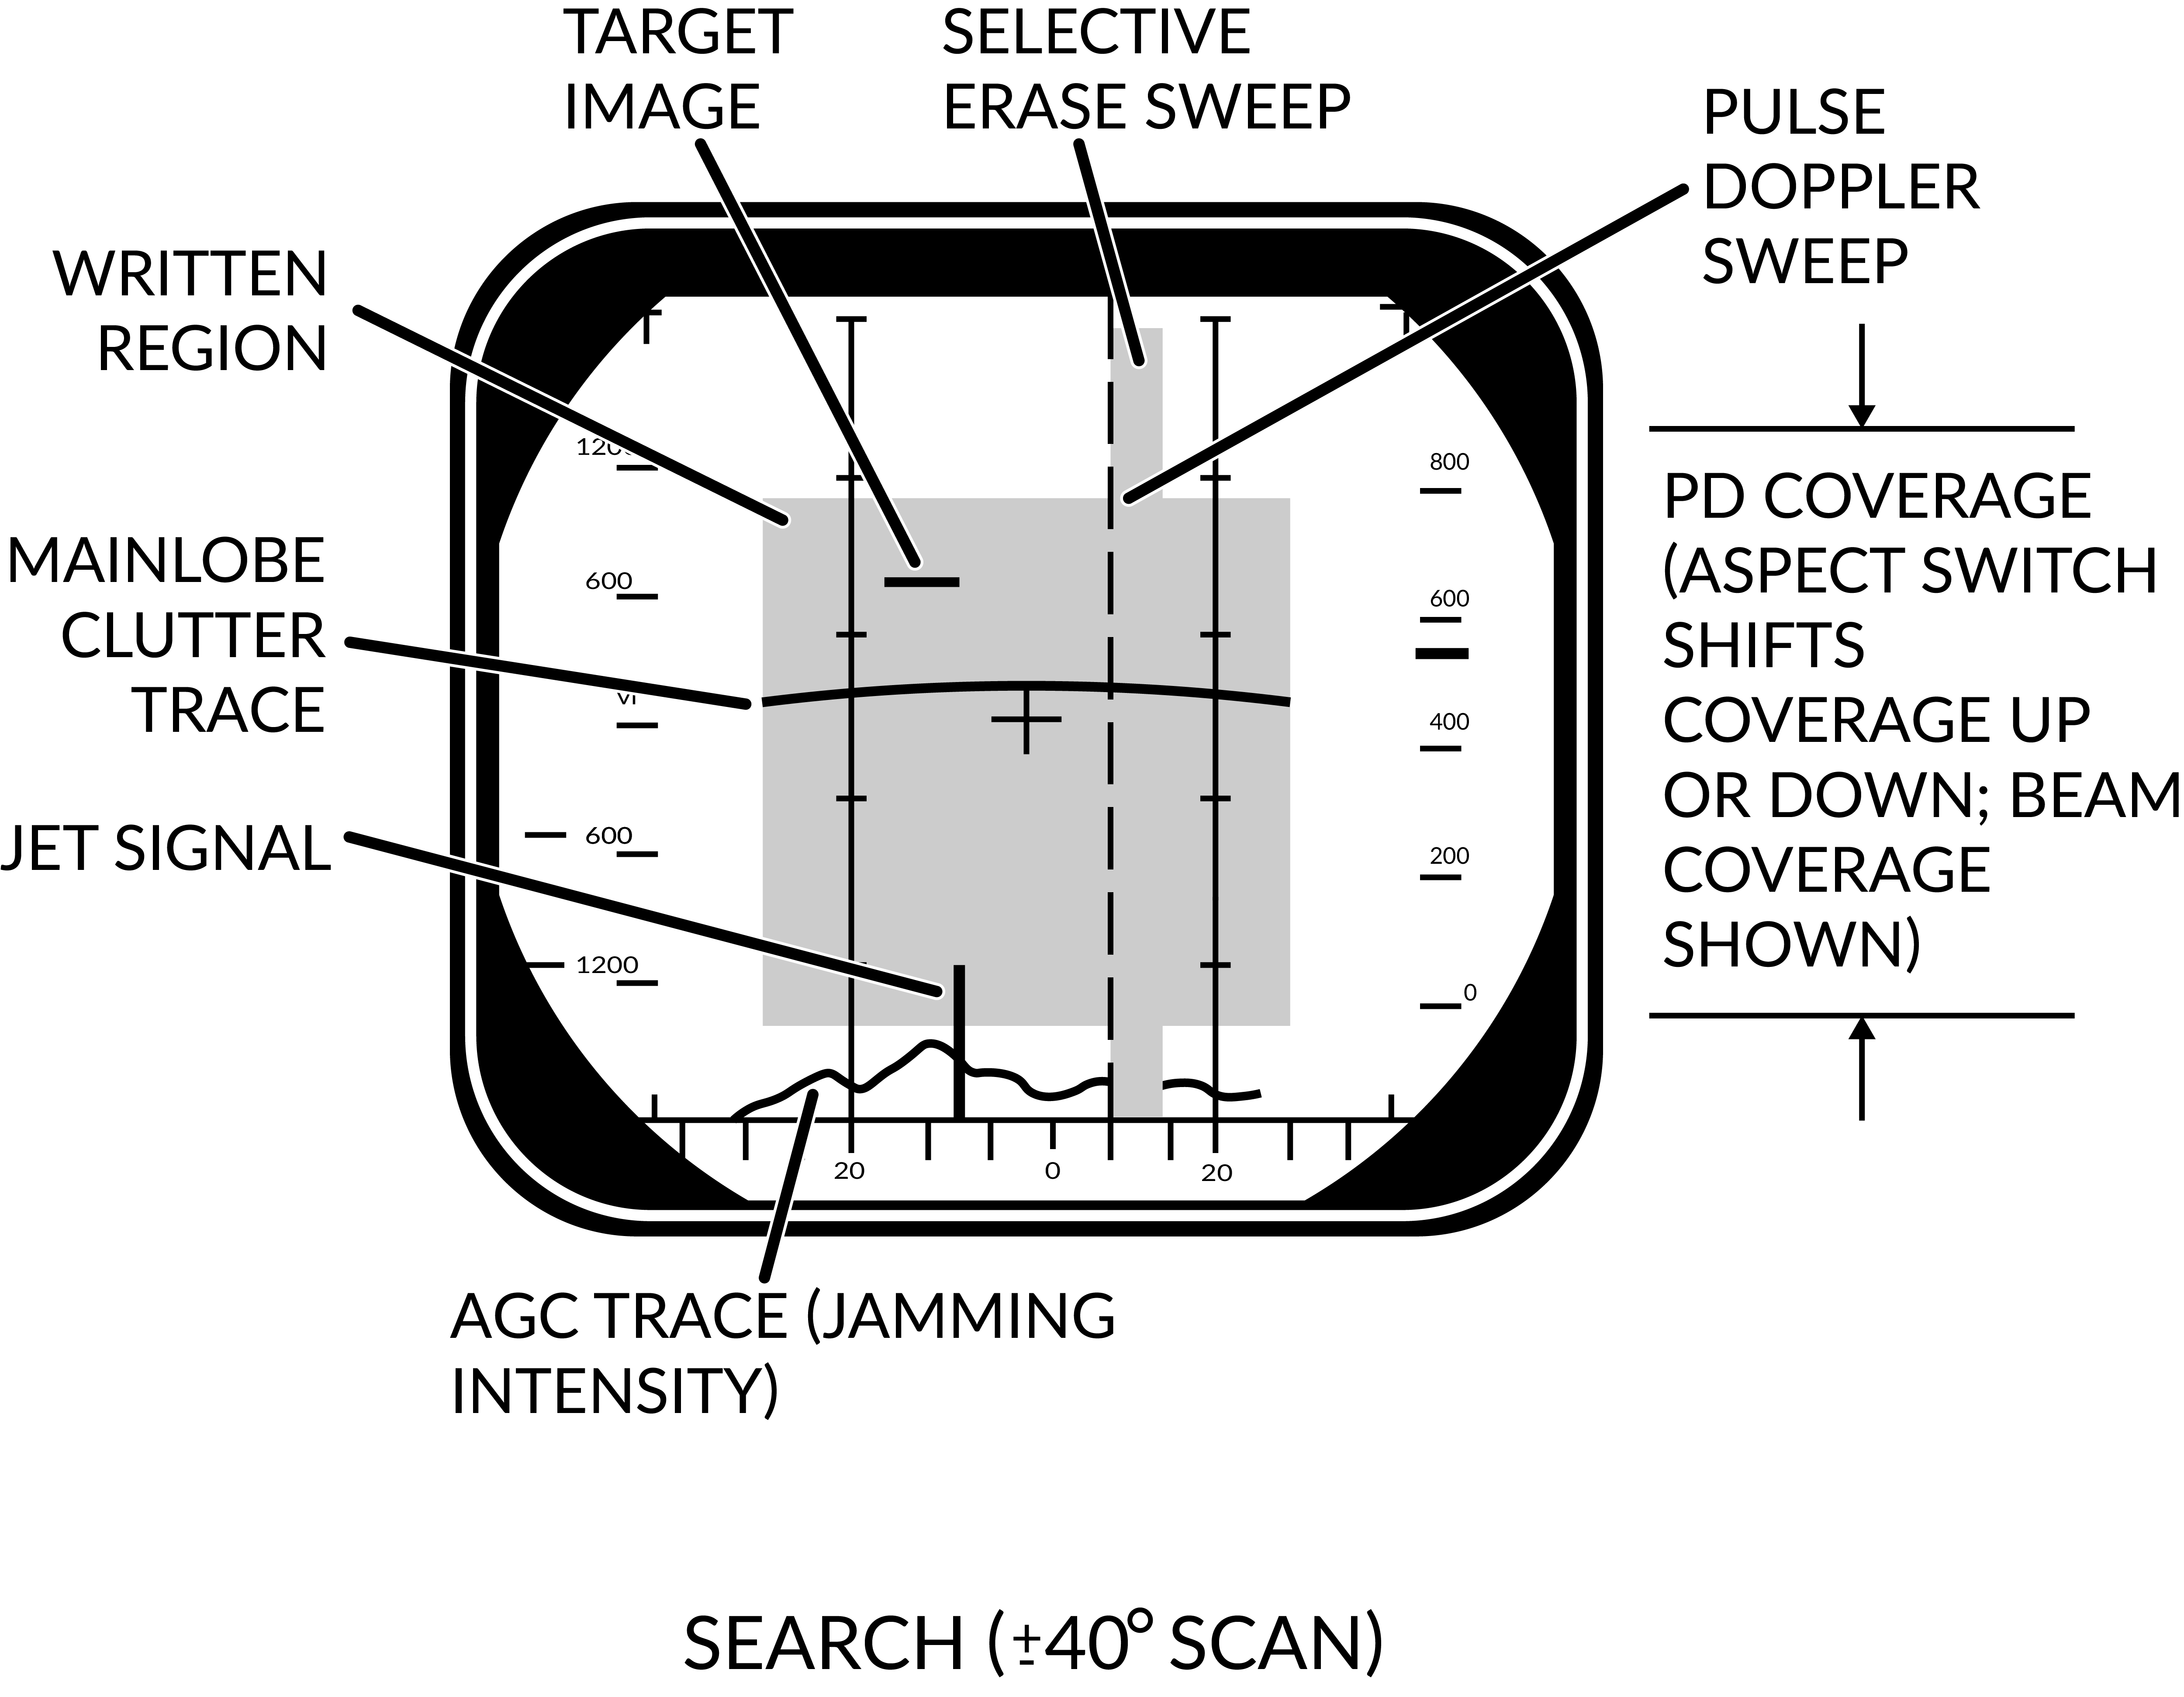
\includegraphics[width=0.9\linewidth]{PDSEARCH.png}
    \caption{\textbf{DDD Format in PD Search Mode}}
    \label{fig:pdsearch}
\end{figure}
\begin{tableitemize}
    \blueitem{Pulse Doppler Search}{ \textbf{``Early Warning'' Mode} - Longest Range, cannot display range

    \begin{subitemize}
        \item \textbf{Advantages}
        \begin{itemize}
            \item Longest Range
            \item Doppler Filtering
            \item \textbf{``Look Down Shoot Down''}
        \end{itemize}
        \item \textbf{Disadvantages}
        \begin{itemize}
            \item Can be notched
            \item No range information
        \end{itemize}
    \end{subitemize}}
    \blueitem{DDD}{
    \begin{subitemize}
        \item \textbf{Closure Rate/Azimuth}
        \item Visualization of radar and erase sweeps
    \end{subitemize}}
    \blueitem{Doppler Filters}{
    \begin{subitemize}
        \item \textbf{MLC -- Main Lobe Clutter Filter}
        \begin{itemize}
            \item \textbf{Own GS +/- 133 knots}
            \item Removes main ground return
            \item Source of notching
        \end{itemize}
        \item \textbf{ZD -- Zero Doppler Filter}
        \begin{itemize}
            \item \textbf{Negative own GS +/- 100 knots}
            \item Removes Radar reflection from ground directly beneath own AC
        \end{itemize}
    \end{subitemize}}
    \dblueitem{MLC Switch}{
    \begin{subitemize}
        \item \textbf{IN:} Enables MLC filter
        \item \textbf{AUTO:} Enables MLC filter if look-up angle less than 3 deg
        \item \textbf{OUT:} Disables MLC filter
    \end{subitemize}}
    \dblueitem{Vc Switch}{Changes closure rate DDD scale
    \begin{subitemize}
        \item \textbf{X-4:} -800 to 4000 knots
        \item \textbf{NORM:} -200 to 1000 knots
        \item \textbf{VID:} -50 to 250 knots
    \end{subitemize}}
    \blueitem{ASPECT Switch}{Changes closure rate processing scale
    \begin{subitemize}
        \item \textbf{NOSE:} -600 to 1800 knots
        \item \textbf{BEAM:} -1200 to 1200 knots
        \item \textbf{TAIL:} -1800 to 600 knots
    \end{subitemize}}
\end{tableitemize}

\clearpage

\begin{figure}[htbp]
    \centering
    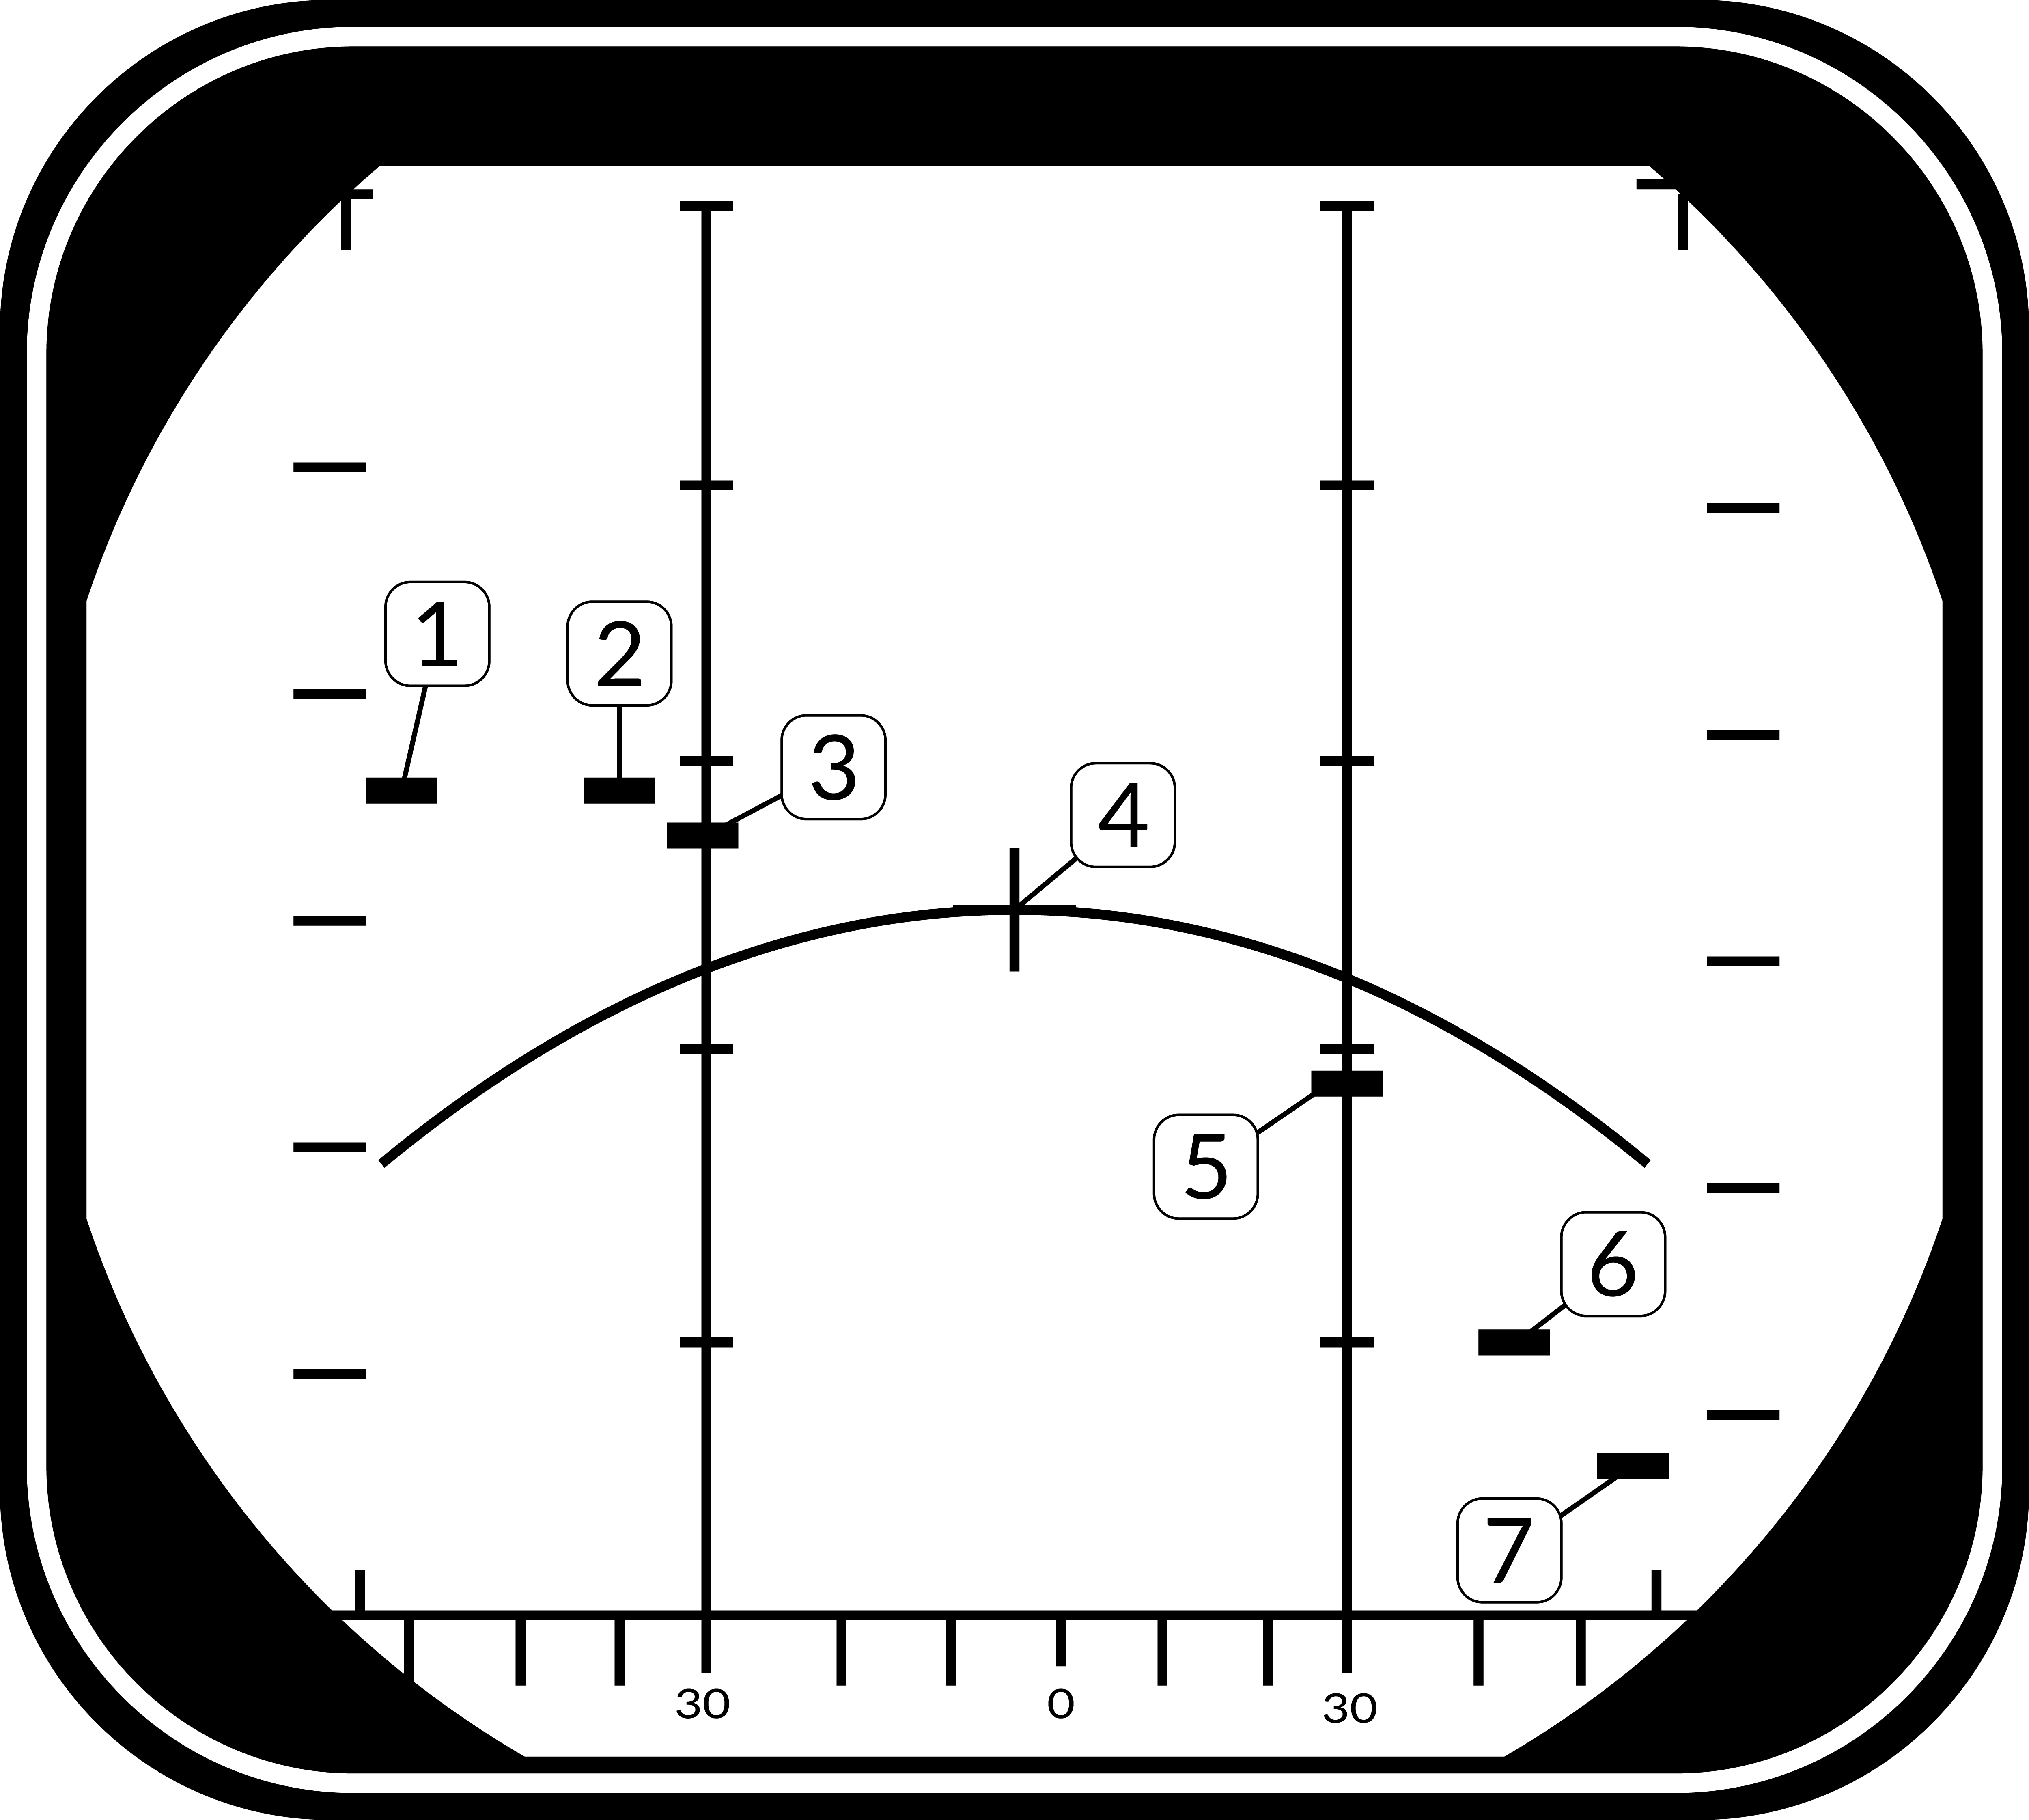
\includegraphics[width=0.5\linewidth]{PD.png}
    \caption{\textbf{DDD Showing Contacts in PD Mode}}
    \label{fig:pd}
\end{figure}
\begin{table}[htbp]
    \centering 
    \caption{\textbf{Target Data for \Cref{fig:pd}}}
    \label{tab:pddata}
    \begin{longtable}{l | l | l | l}
        \toprule
        & \blue{Look Angle} & \blue{Line of Sight Rate} & \blue{Target Heading} \\
        \midrule
        \textbf{1} & 60 deg & 1490 & 180 deg \\
        \midrule
        \textbf{2} & 45 deg & 1500 & 120 deg \\
        \midrule
        \textbf{3} & 30 deg & 1428 & 100 deg \\
        \midrule
        \textbf{4} & 0 deg & 1200 & 90 deg \\
        \midrule
        \textbf{5} & 30 deg & 672 & 80 deg \\
        \midrule
        \textbf{6} & 45 deg & 210 & 60 deg \\
        \midrule
        \textbf{7} & 60 deg & -300 & 0 deg \\
        \bottomrule
    \end{longtable}
\end{table}

\notebox{
    \begin{itemize}
        \item Target \textbf{4} is \emph{notching} and thus shows no radar return
    \end{itemize}
}

\clearpage


\subsection{RWS}
\label{sec:awg9-rws}
\begin{tableitemize}
    \blueitem{Range While Search}{\textbf{FM Ranging}, used for getting good A/A picture before selecting TWS

    \begin{subitemize}
        \item \textbf{FM Ranging}
        \begin{itemize}
            \item Pulse Doppler with ranging
            \item TID shows momentary tracks with ranges
            \item Processing reduces max range
        \end{itemize}
        \item \textbf{Advantages}
        \begin{itemize}
            \item Long Range
            \item Doppler Filtering
            \item \textbf{``Look Down Shoot Down''}
            \item Signal Processing
        \end{itemize}
        \item \textbf{Disadvantages}
        \begin{itemize}
            \item Can be notched
        \end{itemize}
    \end{subitemize}}
    \blueitem{DDD}{
    \begin{subitemize}
        \item \textbf{Closure Rate/Azimuth}
        \item Visualization of radar and erase sweeps
    \end{subitemize}}
    \blueitem{TID}{
    \begin{subitemize}
        \item \textbf{Momentary Tracks}
        \item Max concurrent tracks: 48
        \item \textbf{Cannot lock targets from TID}
    \end{subitemize}}
    \blueitem{Doppler Filters}{
    \begin{subitemize}
        \item \textbf{MLC -- Main Lobe Clutter Filter}
        \begin{itemize}
            \item \textbf{Own GS +/- 133 knots}
            \item Removes main ground return
            \item Source of notching
        \end{itemize}
        \item \textbf{ZD -- Zero Doppler Filter}
        \begin{itemize}
            \item \textbf{Negative own GS +/- 100 knots}
            \item Removes Radar reflection from ground directly beneath own AC
        \end{itemize}
    \end{subitemize}}
\end{tableitemize}

\clearpage

\subsection{TWS}
\label{sec:awg9-tws}

\begin{tableitemize}
    \blueitem{Track While Scan}{\textbf{Builds Track Files}, high situational awareness, multi-target AIM-54 launch
    
    \begin{subitemize}
        \item \textbf{Track Files}
        \begin{itemize}
            \item AWG-9 builds Trackfiles for contacts
            \item Can launch multiple AIM-54
            \item Processing reduces max range
            \item Can lock targets from TID
        \end{itemize}
        \item \textbf{FM Ranging}
        \begin{itemize}
            \item Pulse Doppler with ranging
            \item TID shows momentary tracks with ranges
            \item Processing reduces max range
        \end{itemize}
        \item \textbf{Advantages}
        \begin{itemize}
            \item Doppler Filtering
            \item \textbf{Multi-Target AIM-54}
        \end{itemize}
        \item \textbf{Disadvantages}
        \begin{itemize}
            \item \textbf{Lowest Range}
            \item Can be notched
        \end{itemize}
    \end{subitemize}}
    \blueitem{DDD}{
    \begin{subitemize}
        \item \textbf{Closure Rate/Azimuth}
        \item Visualization of radar and erase sweeps
    \end{subitemize}}
    \blueitem{TID}{
    \begin{subitemize}
        \item \textbf{Tracksfiles}
        \item Max concurrent tracks: 24
        \item Max displayed tracks: 18
    \end{subitemize}}
    \blueitem{Doppler Filters}{
    \begin{subitemize}
        \item \textbf{MLC -- Main Lobe Clutter Filter}
        \begin{itemize}
            \item \textbf{Own GS +/- 133 knots}
            \item Removes main ground return
            \item Source of notching
        \end{itemize}
        \item \textbf{ZD -- Zero Doppler Filter}
        \begin{itemize}
            \item \textbf{Negative own GS +/- 100 knots}
            \item Removes Radar reflection from ground directly beneath own AC
        \end{itemize}
    \end{subitemize}}
    \blueitem{Scan Volume}{Trackfiles require update every 2.5 s -->
    \begin{subitemize}
        \item 20 deg 4 bar (if selected)
        \item 40 deg 2 bar (else)
    \end{subitemize}}
    \blueitem{TID Mode \break Selector}{
    \begin{subitemize}
        \item \textbf{GND STAB:} Ground Stabilized, True North is up on TID
        \item \textbf{A/C STAB:} Aircraft Stabilized
        \item \textbf{ATTAK:} same as A/C STAB with superimposed attack steering symbology
        \item \textbf{TV:} Displays TCS on TID, dispays LANTIRN on TID if equipped
    \end{subitemize}}
    \blueitem{TID Display Selector \break Buttons}{
    \begin{subitemize}
        \item \textbf{RID DISABLE:} Not simulated
        \item \textbf{ALT NUM:} Enables display of track altitudes on left side of track symbols
        \item \textbf{SYM ELEM:} Enables display of all supplementary symbology of tracks and waypoints
        \item \textbf{DATA LINK:} Enables display of D/L contacts
        \item \textbf{JAM STROBE:} Enables display of jam strobes
        \item \textbf{NON-ATTK:} enables/disables display of targets not possible to engage (friendlies)
        \item \textbf{LAUNCH ZONE:} Enables display of weapon launch zones
        \item \textbf{VEL VECTOR:} Enables display of velocity vectors
    \end{subitemize}}
    \blueitem{TRACK HOLD \break CLSN Steering \break Buttons}{
    \begin{subitemize}
        \item \textbf{TRACK HOLD}
        \begin{itemize}
            \item Normally: Tracks maintained for 14 s after last observation
            \item Track Hold: maintained for 2 min after last observation
        \end{itemize}
        \item \textbf{CLSN Button}
        \begin{itemize}
            \item begins collision steering to currently tracked target
            \item enables Steering Centroid if in TWS
            \item LD CLSN presents azimuth steering only
            \item CLSN presents both azimuth and elevation steering
        \end{itemize}
    \end{subitemize}}
    \blueitem{TWS AUTO / MAN}{
    \begin{subitemize}
        \item \textbf{TWS MAN:} Manual azimuth/elevation control, target designation by RIO
        \item \textbf{TWS AUTO:} Automatic prioritization of targets and azimuth elevation control
    \end{subitemize}}
\end{tableitemize}

\clearpage

\subsection{TWS MAN}
\begin{tableitemize}
    \blueitem{TWS MAN}{
    \begin{subitemize}
        \item \textbf{Target Selection:} Manual
        \item \textbf{Scan Azimuth/Elevation:} Manual
    \end{subitemize}}
    \blueitem{Target Selection}{
    \begin{subitemize}
        \item \textbf{Conditions}
        \begin{itemize}
            \item TWS MAN Radar Mode selected
            \item TID CURSOR TID Mode selected
        \end{itemize}
        \item \textbf{Hook Target}
        \begin{enumerate}
            \item Hold HCU Half-Action
            \item Slew TID Cursor over desired Tgt
            \item HCU Full-Action to select Tgt
        \end{enumerate}
        \item \textbf{TID Symbology}
        \begin{itemize}
            \item Range (\textbf{RA})
            \item Bearing (\textbf{BR})
            \item Altitude (\textbf{AL})
            \item Magnetic course (\textbf{MC})
        \end{itemize}
        \item \textbf{Lock Target}
        \begin{enumerate}[label=(\alph*), resume]
            \item Press \textbf{PD STT} or \textbf{Pulse STT} buttons
        \end{enumerate}
        \item \textbf{Deselect Target}
        \begin{enumerate}[label=(\alph*), resume]
            \item press HCU Half-Action
        \end{enumerate}
    \end{subitemize}}
    \blueitem{AIM-54 Launch}{
    \begin{subitemize}
        \item \textbf{Automatically selects TWS AUTO}
        \item \textbf{Prevents selection of TWS MAN}
    \end{subitemize}}
\end{tableitemize}

\clearpage

\subsection{TWS AUTO}
\begin{tableitemize}
    \blueitem{TWS AUTO}{
    \begin{subitemize}
        \item \textbf{Target Selection:} prioritizes contacts based off range, aspect, closure
        \item \textbf{Scan Azimuth/Elevation:} Geometric center of targets in scan volume
    \end{subitemize}}
    \blueitem{Centroid / Steering Cues}{
    \begin{subitemize}
        \item \textbf{Steering Centroid}
        \begin{itemize}
            \item facilitates steering cues
            \item HUD, VDI, TID, DDD
            \item Appears as \textbf{X} on TID
            \item Takes Gimbal limits into account
            \item Weights individual Tracks based on parameters
        \end{itemize}
        \item \textbf{Illumination Centroid}
        \begin{itemize}
            \item \textbf{Not Visible}
            \item Controls azimuth and elevation of scan pattern
            \item Takes scan volume into account
        \end{itemize}
    \end{subitemize}}
    \blueitem{Pilot Steering Cues}{
    \begin{subitemize}
        \item \textbf{Conditions}
        \begin{itemize}
            \item A-A HUD Mode selected
            \item Master Arm ON (UP)
            \item AIM-54 or AIM-7 selected
            \item TWS-AUTO selected
        \end{itemize}
    \end{subitemize}}
\end{tableitemize}

\clearpage

\subsection{PDSTT}
\begin{figure}[htbp]
    \centering
    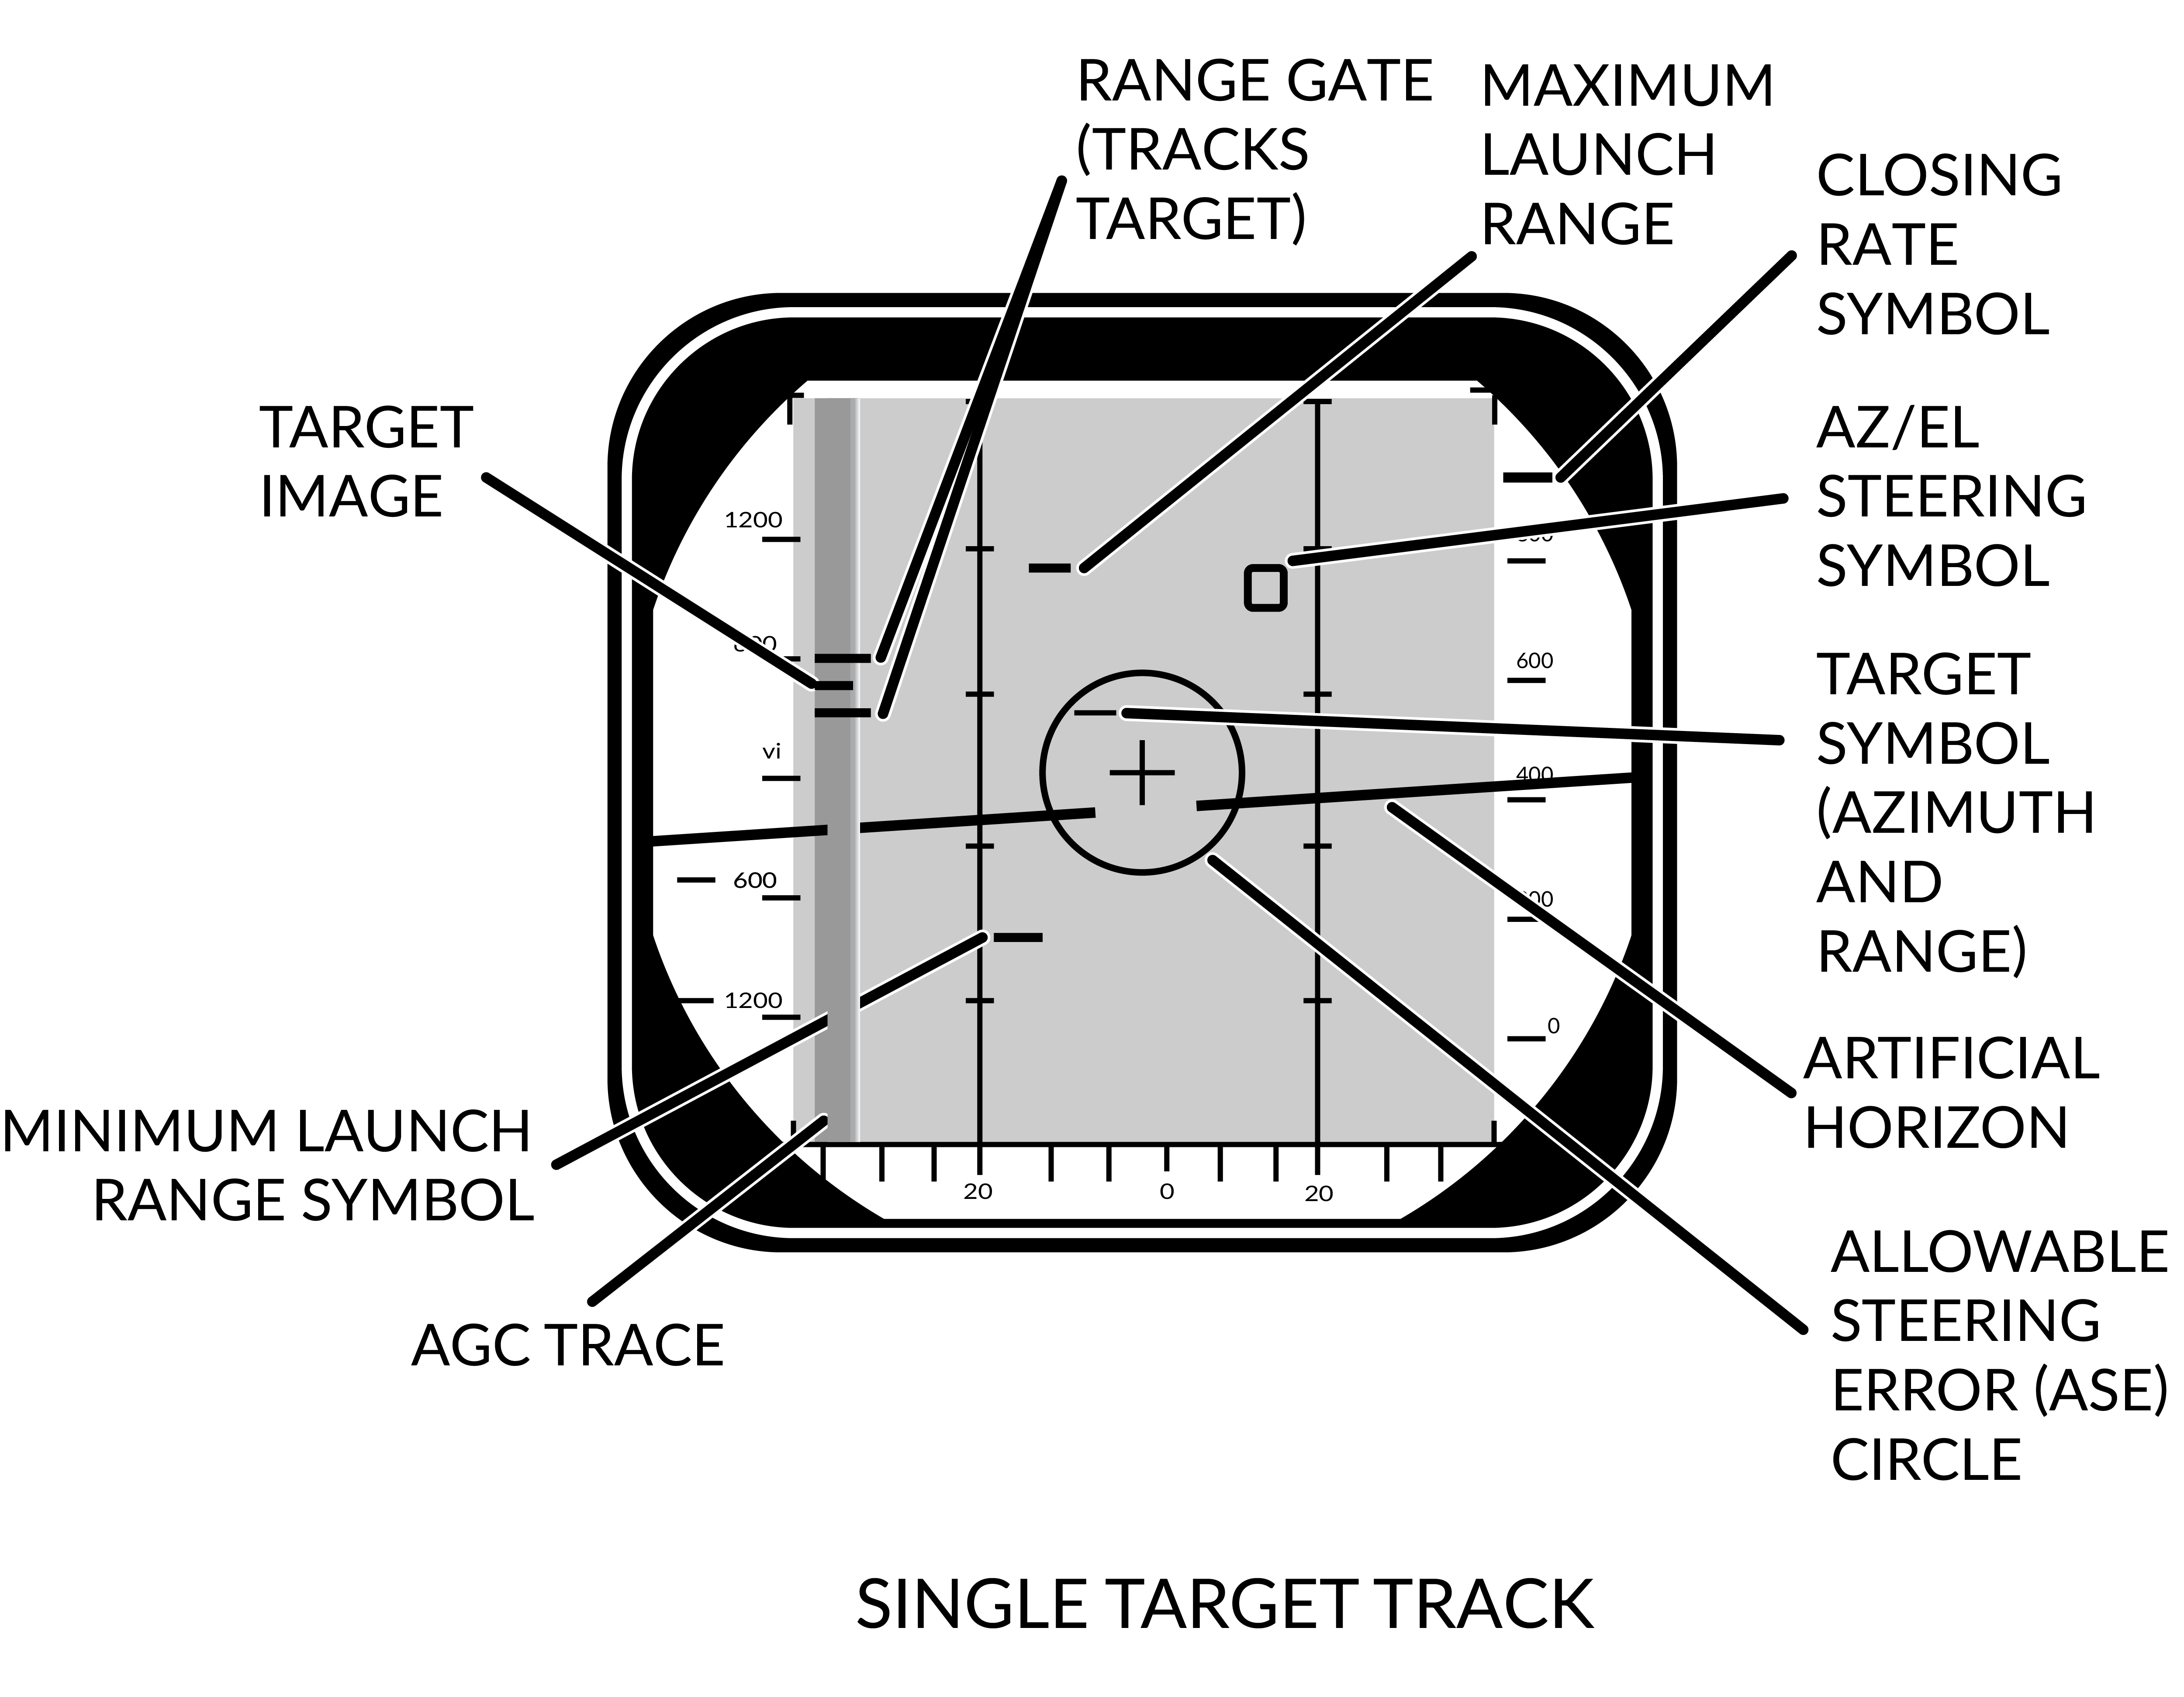
\includegraphics[width=0.9\linewidth]{PDSTT.png}
    \caption{\textbf{DDD Format in PDSTT Mode}}
    \label{fig:pdstt}
\end{figure}
\begin{tableitemize}
    \blueitem{Pulse Doppler STT}{
    \begin{subitemize}
        \item \textbf{Advantages} -- Ground Clutter filtering
        \item \textbf{Disadvantages} -- Susceptible to notching
    \end{subitemize}}
    \blueitem{DDD}{
    \begin{subitemize}
        \item \textbf{Track Indications}
        \begin{itemize}
            \item ANT TRK \& RDROT lights
            \item Tracking gates
            \item Closure rate
            \item Attack Symbology
        \end{itemize}
    \end{subitemize}}
\end{tableitemize}

\notebox{
    \begin{itemize}
        \item \textbf{PDSTT Lock Affects Missile Logic}
        \begin{itemize}
            \item Enables launch of AIM-54/AIM-7 in \textbf{PD Mode}
            \item AIM-7 PD launch requires \textbf{MSL OPTIONS Switch} to be in \textbf{SP PD}  
        \end{itemize}
    \end{itemize}
}

\clearpage

\subsection{PDSTT ACQUISITION}
\begin{tableitemize}
    \blueitem{PD To PDSTT}{
    \begin{subitemize}
        \item \textbf{Conditions}
        \begin{itemize}
            \item PD Search Mode selected
            \item RDR HCU Mode selected
        \end{itemize}
        \item \textbf{Lock Target}
        \begin{enumerate}
            \item Hold HCU Half-action
            \item Slew acquisition gates over desired Target on DDD
            \item HCU Full-Action to lock
        \end{enumerate}
        \item \textbf{Unlock Target}
        \begin{enumerate}[resume]
            \item HCU Half-action
        \end{enumerate}
    \end{subitemize}}
    \blueitem{TWS to PDSTT}{
    \begin{subitemize}
        \item \textbf{Conditions}
        \begin{itemize}
            \item TWS Mode selected
            \item RDR HCU Mode selected
        \end{itemize}
        \item \textbf{Lock Target}
        \begin{enumerate}
            \item Hook Target on TID
            \item Press PDSTT button on DDD Panel
        \end{enumerate}
        \item \textbf{Unlock Target}
        \begin{enumerate}[resume]
            \item HCU Half-action
        \end{enumerate}
    \end{subitemize}}
    \blueitem{PSTT to PDSTT}{
    \begin{subitemize}
        \item \textbf{Conditions}
        \begin{itemize}
            \item Target PSTT Locked
        \end{itemize}
        \item \textbf{Lock Target}
        \begin{enumerate}
            \item Press PDSTT button on DDD Panel
        \end{enumerate}
        \item \textbf{Unlock Target}
        \begin{enumerate}[resume]
            \item HCU Half-action
        \end{enumerate}
    \end{subitemize}}
\end{tableitemize}

\clearpage

\section{ACM MODES}
\subsection{OVERVIEW}
\begin{center}
    \begin{tabular}{p{3cm} | p{2cm}  | p{2cm} | p{2cm} | p{2cm}}
        \toprule
        & \blue{PLM} & \blue{VSL} & \blue{PAL} & \blue{MRL} \\
        \midrule
        \textbf{Range} & 5 nm & 5 nm & 15 nm & 5 nm \\
        \midrule
        \textbf{Description} & Boresight & Vertical & Horizontal & RIO \\
        \midrule
        \textbf{Weapons} & \multicolumn{4}{c}{Gun + All Missiles} \\
        \bottomrule
    \end{tabular}
\end{center}

\begin{tableitemize}
    \blueitem{PLM}{
    \begin{subitemize}
        \item \textbf{Pilot Lockon Mode} -- see \Cref{fig:acmvisplm}
        \item \textbf{Highest Priority ACM}
        \item \textbf{Search Pattern}
        \begin{itemize}
            \item Small Boresight
            \item Range: 5 nm
        \end{itemize}
    \end{subitemize}}
    \blueitem{VSL}{
    \begin{subitemize}
        \item \textbf{Vertical Scan Lockon} -- see \Cref{fig:acmvisvsl}
        \item \textbf{HI Search Pattern}
        \begin{itemize}
            \item Width: 5 deg
            \item Vertical: +15 to +55 deg
            \item Range: 5 nm
        \end{itemize}
        \item \textbf{LO Search Pattern}
        \begin{itemize}
            \item Width: 5 deg
            \item Vertical: -15 to +25 deg
            \item Range: 5 nm
        \end{itemize}
        \item \textbf{RIO/PILOT Controlled}
    \end{subitemize}}
    \blueitem{PAL}{
    \begin{subitemize}
        \item \textbf{Pilot Automatic Lockon}
        \item \textbf{Search Pattern}
        \begin{itemize}
            \item Width: +/- 20 deg
            \item Vertical: 8-bar
            \item Range: 15 nm
        \end{itemize}
    \end{subitemize}}
    \blueitem{MRL}{
    \begin{subitemize}
        \item \textbf{Manual Rapid Lockon} -- see \Cref{fig:acmvismrl}
        \item \textbf{RIO Controlled}
        \item \textbf{Search Pattern}
        \begin{itemize}
            \item HCU Controlled
            \item Range: 5 nm
        \end{itemize}
    \end{subitemize}}
\end{tableitemize}

\notebox{
    \begin{itemize}
        \item \textbf{ACM Modes Result in PSTT Lock} -- affects missile logic
        \begin{itemize}
            \item AIM-54 launched in \textbf{Active Launch Mode}
            \item AIM-7 launched in \textbf{CW Mode}
        \end{itemize}
    \end{itemize}
}
\warningbox{
    \begin{itemize}
        \item \textbf{Active Launch Mode Phoenixes Have Limited IFF Capability} 
        \begin{itemize}
            \item Employ with caution when friendlies airborne
        \end{itemize}
    \end{itemize}
}

\begin{figure}[htbp]
    \centering
    \begin{subfigure}[c]{0.55\linewidth}
        \centering
        \includegraphics[width=0.8\linewidth]{PLM.png}
        \subcaption{\textbf{PLM Search Pattern}}
        \label{fig:acmvisplm}
        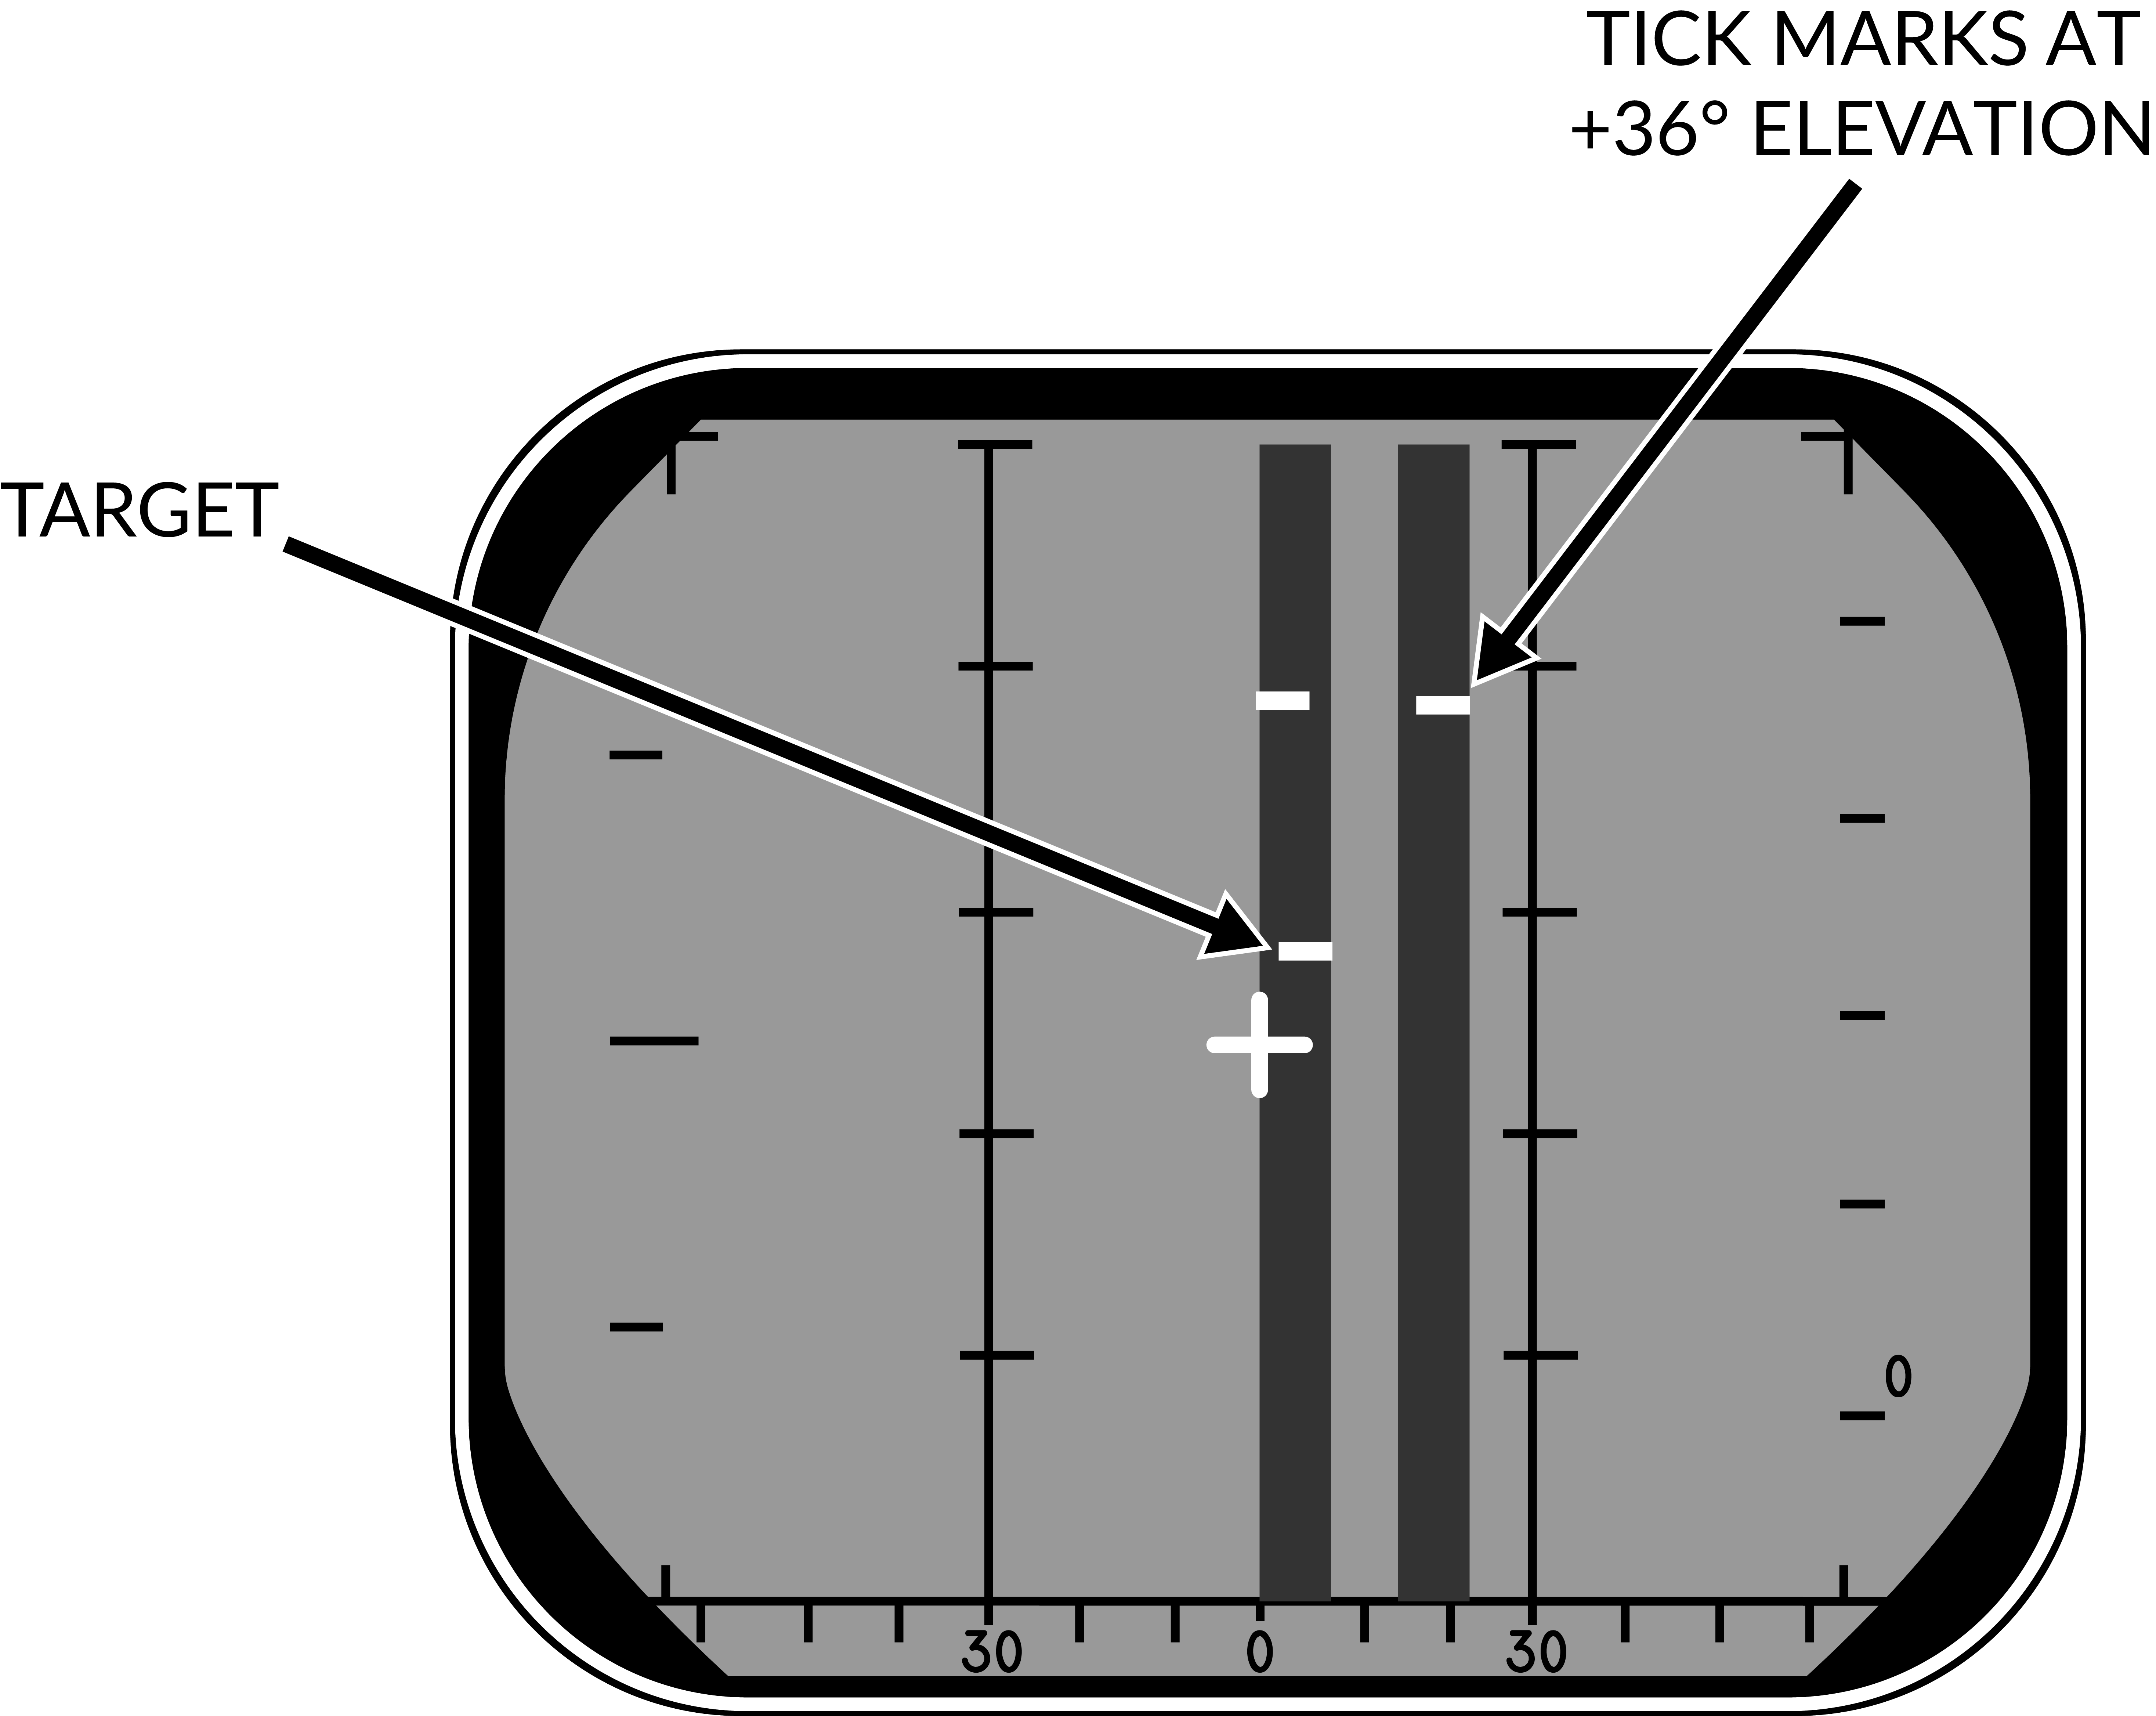
\includegraphics[width=\linewidth]{mrl.png}
        \subcaption{\textbf{DDD Format in MRL Mode}}
        \label{fig:acmvismrl}
    \end{subfigure}
    \begin{subfigure}[c]{0.43\linewidth}
        \centering
        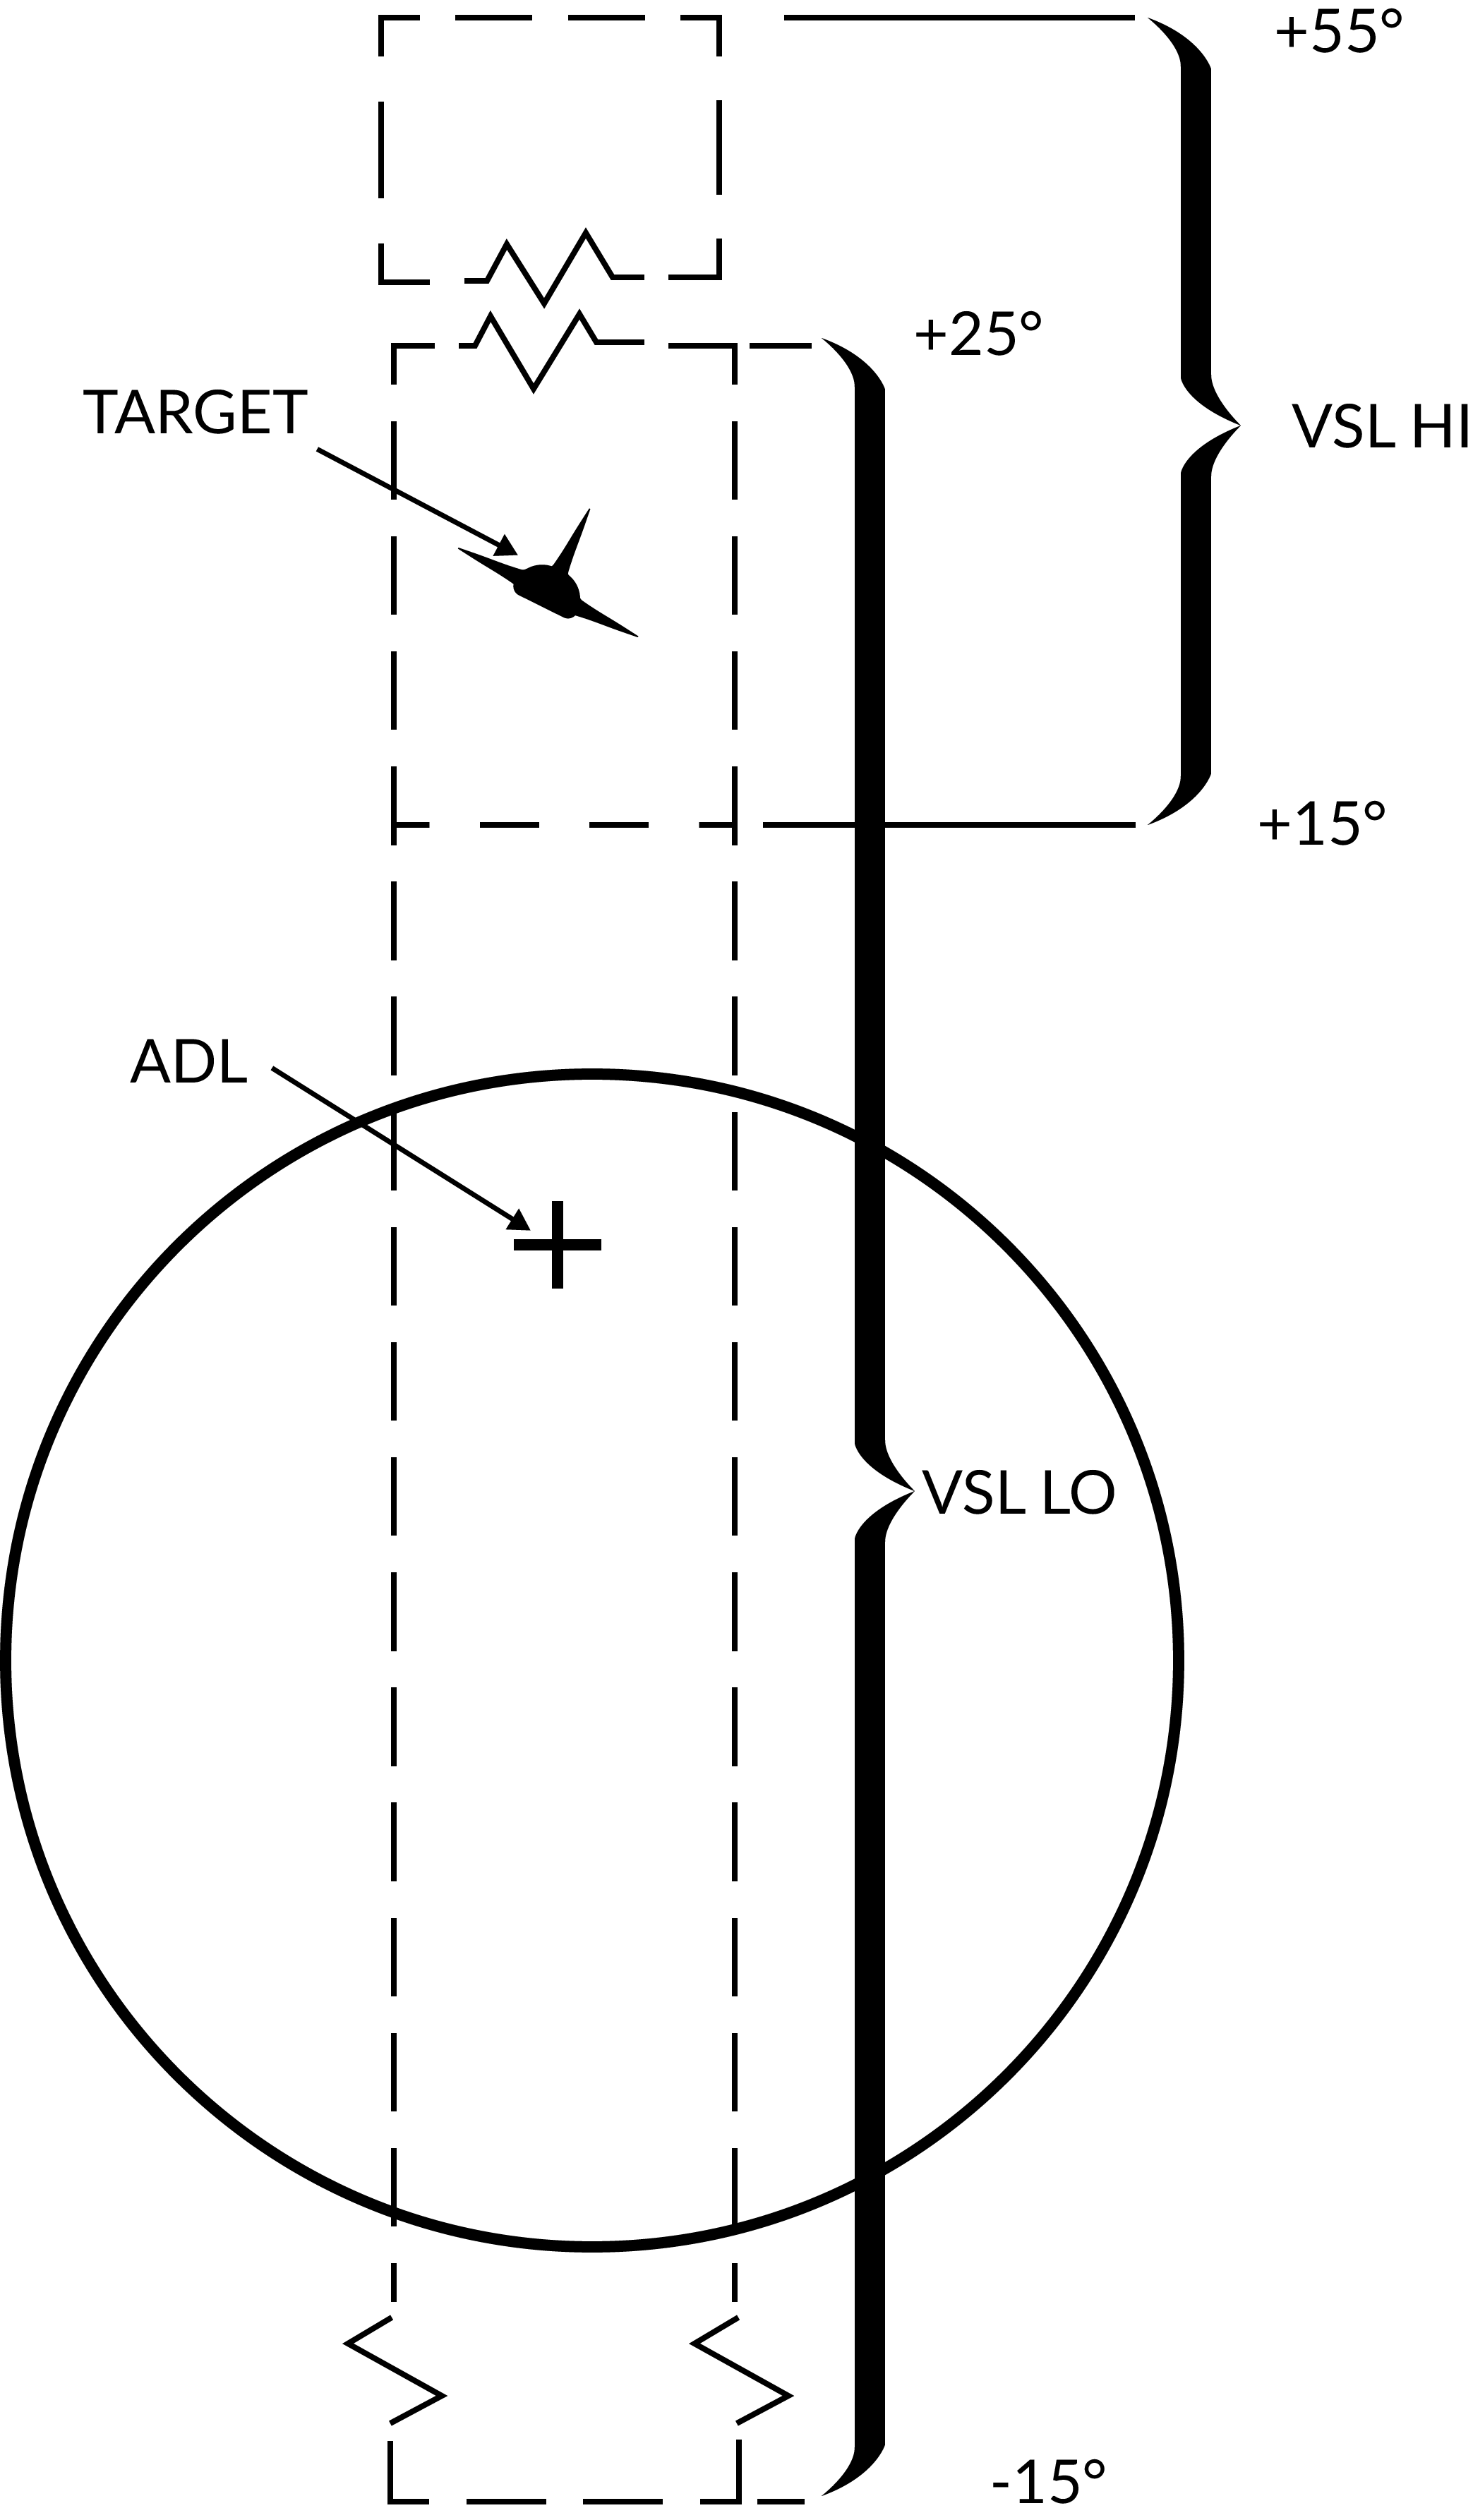
\includegraphics[width=\linewidth]{vsl.png}
        \subcaption{\textbf{VSL Search Patterns}}
        \label{fig:acmvisvsl}
    \end{subfigure}
    \caption{\textbf{ACM Search Mode Visualization}}
    \label{fig:acmvis}
\end{figure}

\clearpage 

\section{APX-76 IFF}
\subsection{OVERVIEW}
\begin{tableitemize}
    \blueitem{Activation}{\textbf{IFF Switch} -- \textbf{Press \& Hold} (up to 10 sec)}
    \blueitem{Search Modes}{
        \begin{subitemize}
            \item \textbf{DDD} -- 2 horizontal bars above \& below all friendly returns
        \end{subitemize}
    }
    \blueitem{TWS / STT Modes}{
        \begin{subitemize}
            \item \textbf{DDD} -- 2 horizontal bars above \& below hooked / locked friendly 
            \item \textbf{DDD Range} -- shows \textbf{10 EXP}
        \end{subitemize}
    }
    \blueitem{Control Panel}{\textbf{Non-Functional in DCS} -- it \emph{just works}}
\end{tableitemize}

\notebox{
    \begin{itemize}
        \item \textbf{APX-76 Data is Not Correlated with TWS Tracks} -- RIO must manually enter target status (HOST, UNKN, FRIEND) via the \textbf{CAP}
        \item \textbf{Lack of IFF Return does NOT necessarily mean Hostile} 
        \item \textbf{APX-76 is a Secondary, Transponder-type Radar}
        \begin{itemize}
            \item Can receive IFF returns from targets not detected by AWG-9
        \end{itemize}
    \end{itemize}
}